\documentclass[12pt]{article}
\usepackage[utf8]{inputenc}
\usepackage{amsmath, amssymb, amsthm, graphicx, fancyvrb, enumitem, titlesec, setspace, float, fancyvrb, minted}
\usepackage[dvipsnames]{xcolor}
\usepackage[top=1in, bottom=1in, left=1.25in, right=1.25in]{geometry}
\titleformat{\section}{\normalfont\bfseries}{}{0em}{}
\titlespacing*{\section}{0pt}{1.5ex plus .2ex minus .2ex}{0.8ex plus .1ex}


\begin{document}
\noindent Andre Winkel \hfill \today \\
\rule{\textwidth}{0.4pt} \vspace{0em}
\begin{center} \large{Lab 6} \end{center} \vspace*{0em}

\section*{Problem 1: Understanding low-pass filters}
In this problem, we consider ideal low-pass filter
\begin{equation} \notag
    H_0(e^{j\omega})=
    \begin{cases}
        1 & \frac{-\pi}{10}\le \omega \le \frac{\pi}{10}\\
        0 & \text{otherwise}
    \end{cases}
\end{equation}
which has a time-domain signal
\begin{equation} \notag
    h_0[n]=\frac{1}{10}\text{sinc}(\frac{\pi n}{10})=
    \begin{cases}
        \frac{\sin(\frac{\pi n}{10})}{\pi n} & n\ne0\\
        \frac{1}{10} & n=0
    \end{cases}
\end{equation}
which is neither causal nor finite. In this lab, we will observe the effects of this operation on the magnitude and phase of the filter. 

\begin{enumerate}[label=\textbf{\alph*)}, leftmargin=2.6em]
\item We begin by defining the rectangular pulse as
\begin{equation} \notag
    r[n]=
    \begin{cases}
        1 & -n_0\le n \le n_0\\
        0 & \text{otherwise}
    \end{cases}
\end{equation}
and
\begin{equation} \notag
    h_1[n]=h_0[n-n_0]r[n-n_0]
\end{equation}
with $n_0=10$. Computing and plotting $h_1[n]$, $|H_1(e^{j\omega})|$, and $\angle H_1(e^{jw})$, we observe the following plots:
\begin{figure} [H]
    \centering
    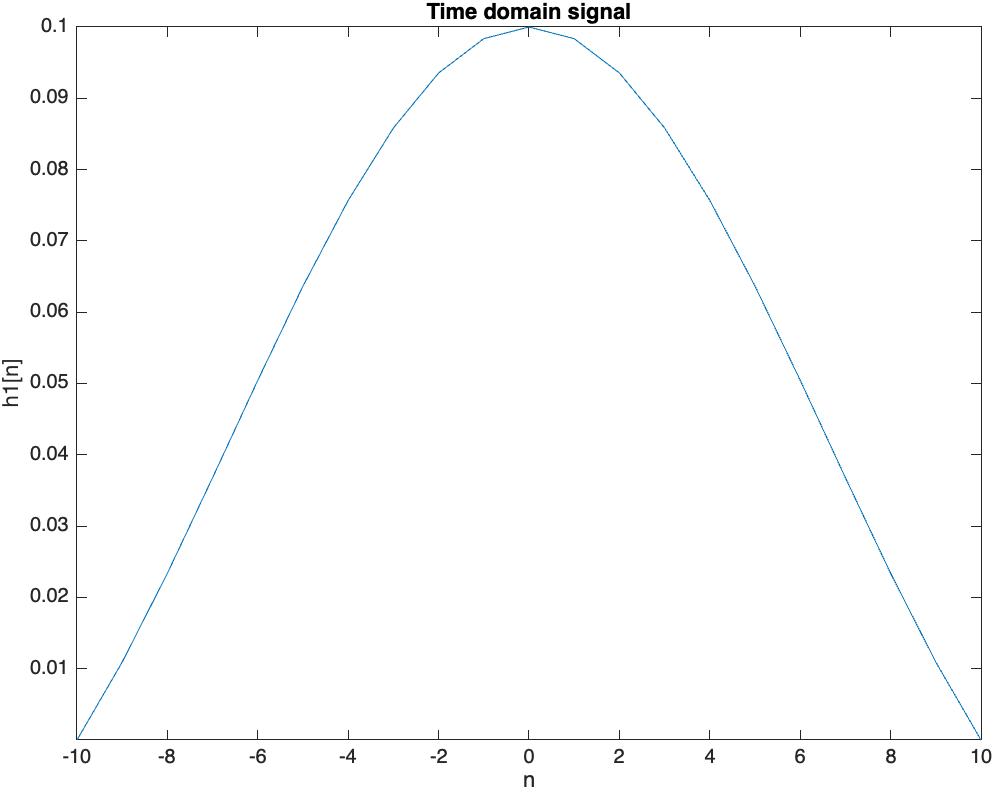
\includegraphics[width=0.75\linewidth]{1.png}
\end{figure}
\begin{figure} [H]
    \centering
    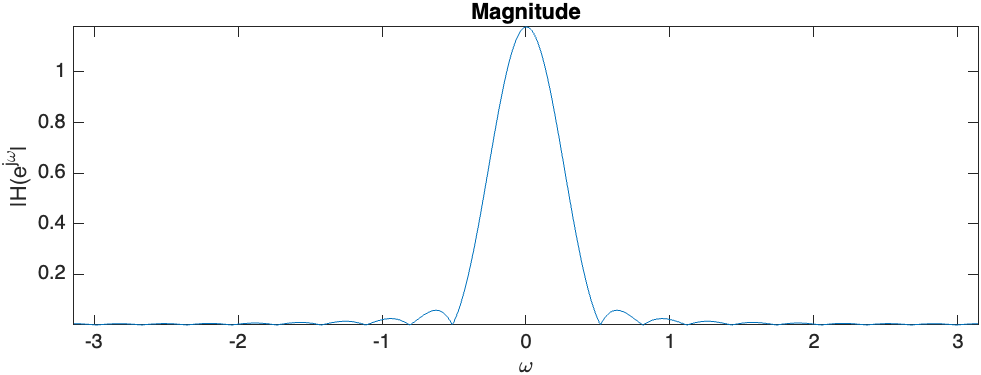
\includegraphics[width=0.75\linewidth]{2.png}
\end{figure}
\begin{figure} [H]
    \centering
    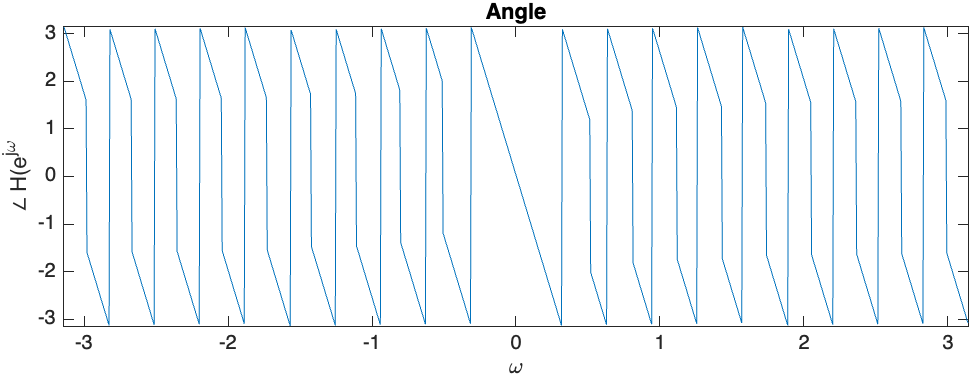
\includegraphics[width=0.75\linewidth]{3.png}
\end{figure}
In the above figures, we observe the plots of the time domain signal $h_1[n]$, as well as the magnitude and phase of the frequency domain representation. We can observe that the magnitude plot is a very rough sinusoidal representation of the ideal low-pass filter, while the phase plot reflects our $n_0$ delay through the wrapped linear plot. It is also important to note the effects of the Gibbs phenomenon being visible in the magnitude plot, though less apparent as we have fewer samples. Doing the same for $n_0=20$, we obtain the following plots:
\begin{figure} [H]
    \centering
    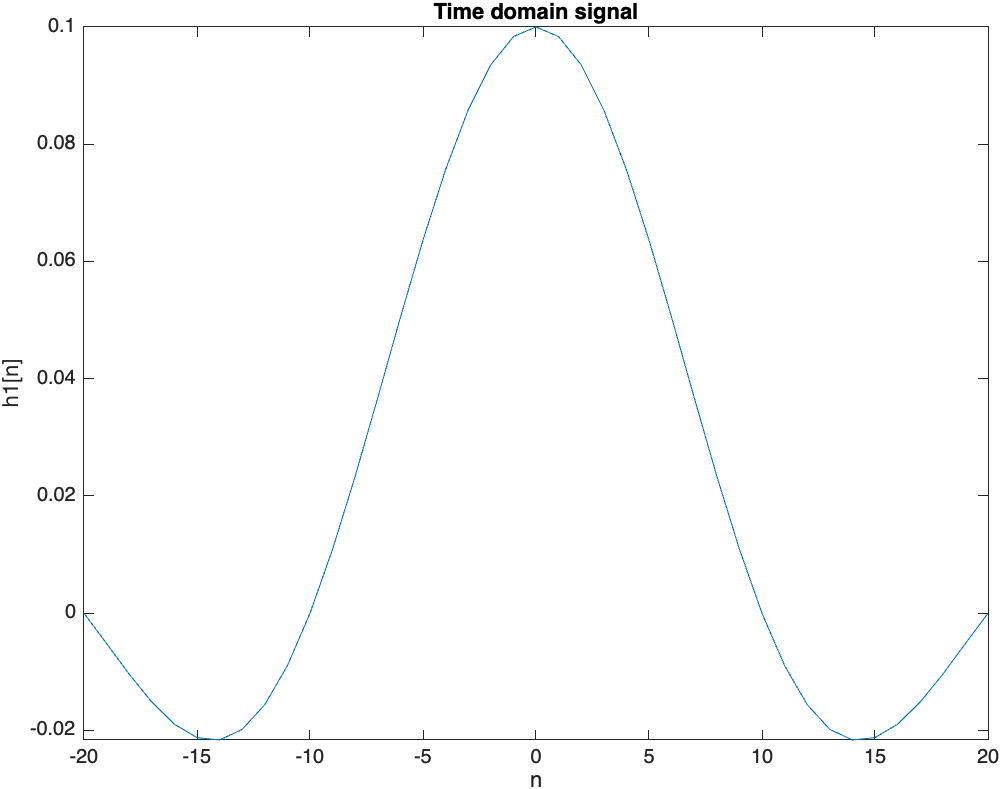
\includegraphics[width=0.75\linewidth]{4.png}
\end{figure}
\begin{figure} [H]
    \centering
    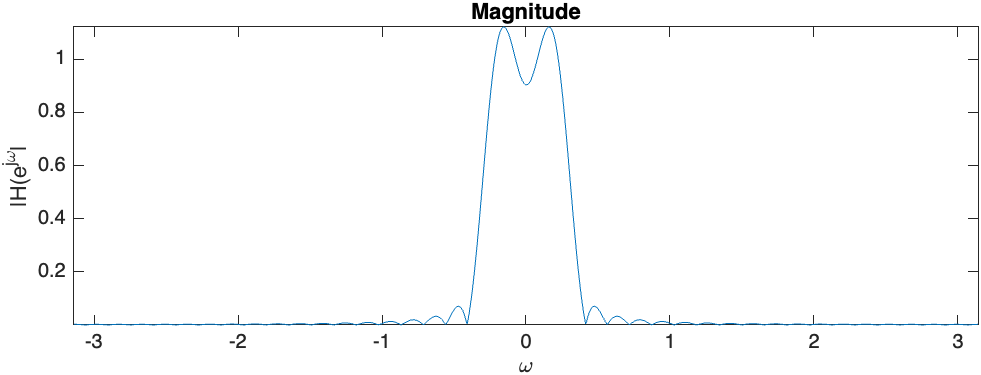
\includegraphics[width=0.75\linewidth]{5.png}
\end{figure}
\begin{figure} [H]
    \centering
    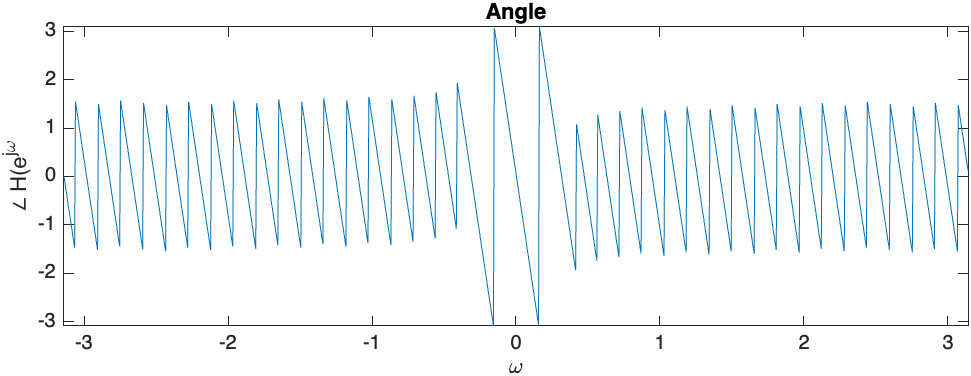
\includegraphics[width=0.75\linewidth]{6.png}
\end{figure}
And again, for $n_0=50$, we see:
\begin{figure} [H]
    \centering
    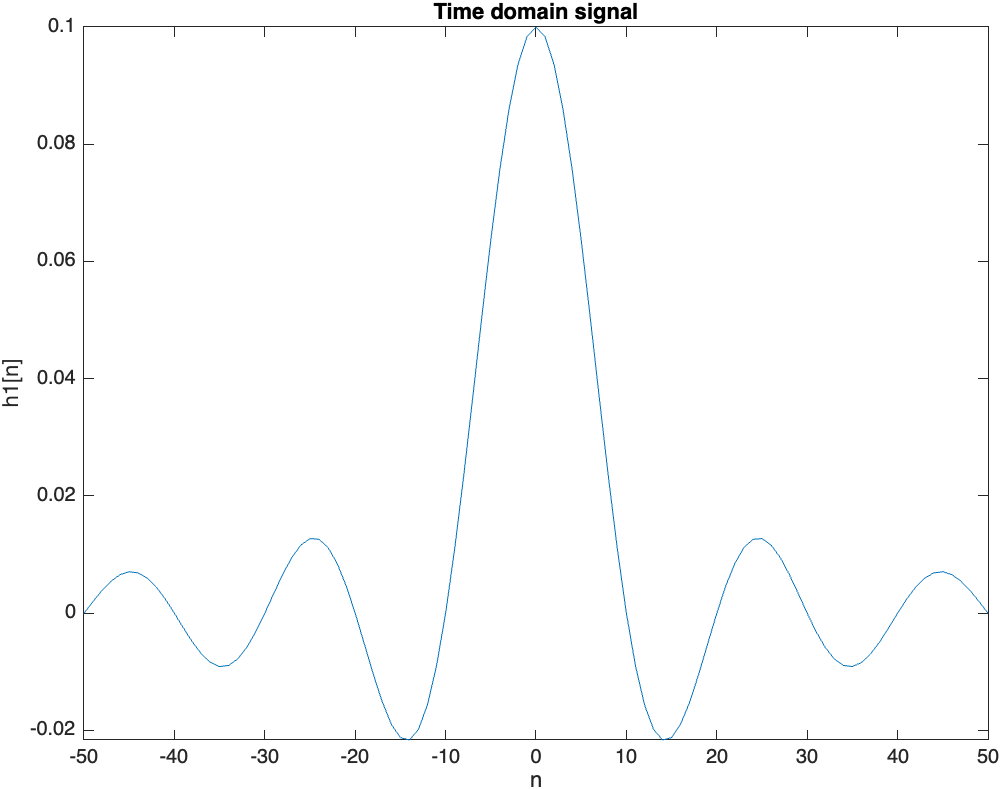
\includegraphics[width=0.75\linewidth]{7.png}
\end{figure}
\begin{figure} [H]
    \centering
    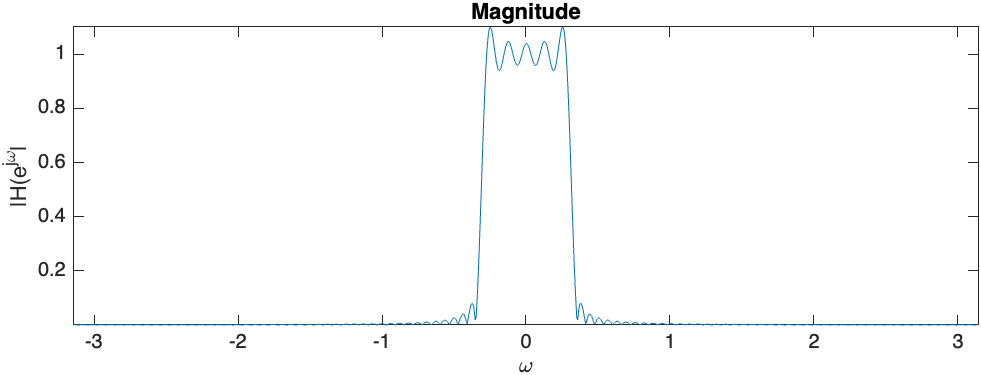
\includegraphics[width=0.75\linewidth]{8.png}
\end{figure}
\begin{figure} [H]
    \centering
    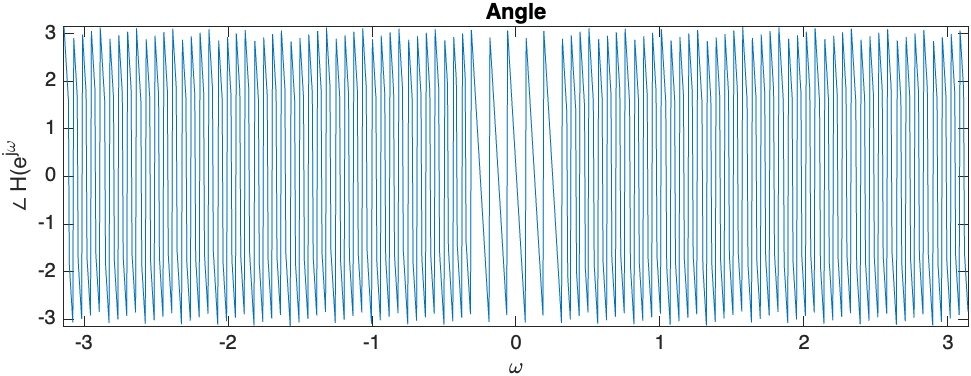
\includegraphics[width=0.75\linewidth]{9.png}
\end{figure}
We can directly observe a higher fidelity in the shape of the original filter magnitude $|H_0(e^{j\omega})|$ as $n_0$ increases, though the Gibbs phenomenon is more apparent. On the other hand, we see $\angle H_1(e^{j\omega})$ becomes much more dense and nearly indecipherable, though this is the behavior that we expect from this plot \--- it resembles the initial phase plot though having many more samples.

\begin{minted}[frame=single, fontsize=\small, linenos, bgcolor=white]{matlab}
% h1[n]=h0[n-n0]r[n-n0]
sinc(0);

n0 = 10;
n = -n0:n0;
h0 = sinc(n/10)/10;

r1 = ones(size(n));
h1 = h0.*r1;

subplot(1, 1, 1);
plot(n, h1);
xlabel('n');
ylabel('h1[n]');
axis tight;
title('Time domain signal')

windowed_resp = h1;
N_fft = 1024;

% fftshift shifts the zero-frequency to center of the array N_fft/2
impulse_resp_fft = fftshift(fft(windowed_resp, N_fft));

% Discrete frequencies
freqs = linspace(-pi, pi, N_fft);
fig1 = figure;

subplot(2, 1, 1);
plot(freqs, abs(impulse_resp_fft));
xlabel('\omega');
ylabel('|H(e^{j\omega}|');
axis tight;
title('Magnitude');

subplot(2, 1, 2);
plot(freqs, angle(impulse_resp_fft));
xlabel('\omega');
ylabel('\angle H(e^{j\omega}');
axis tight;
title('Angle');
\end{minted}

\item Now, we will perform the truncation using the triangular pulse, defined as
\begin{equation} \notag
    t[n]=
    \begin{cases}
        1+\frac{n}{n_0} & -n_0\le n\le 0\\
        1-\frac{n}{n_0} & 0\le n\le n_0\\
        0 & \text{otherwise}
    \end{cases}
\end{equation}
and we let
\begin{equation} \notag
    h_2[n]=h_0[n-n_0]t[n-n_0].
\end{equation}
We then observe the following plots for $n_0=10$:
\begin{figure} [H]
    \centering
    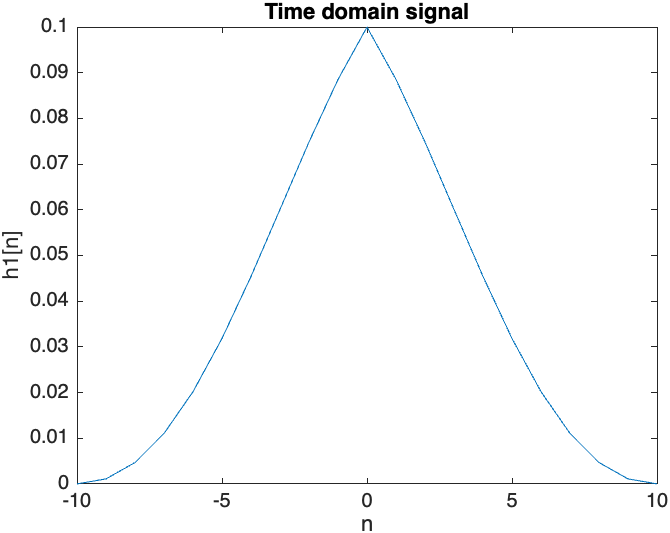
\includegraphics[width=0.75\linewidth]{10.png}
\end{figure}
\begin{figure} [H]
    \centering
    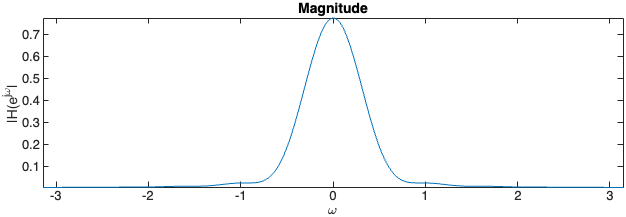
\includegraphics[width=0.75\linewidth]{11.png}
\end{figure}
\begin{figure} [H]
    \centering
    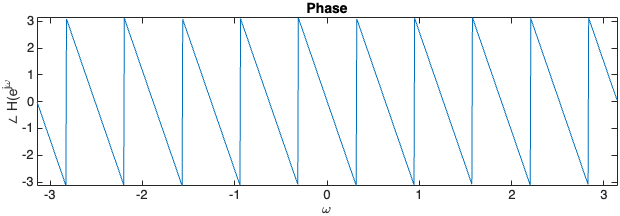
\includegraphics[width=0.75\linewidth]{12.png}
\end{figure}
And for $n_0=20$, we see:
\begin{figure} [H]
    \centering
    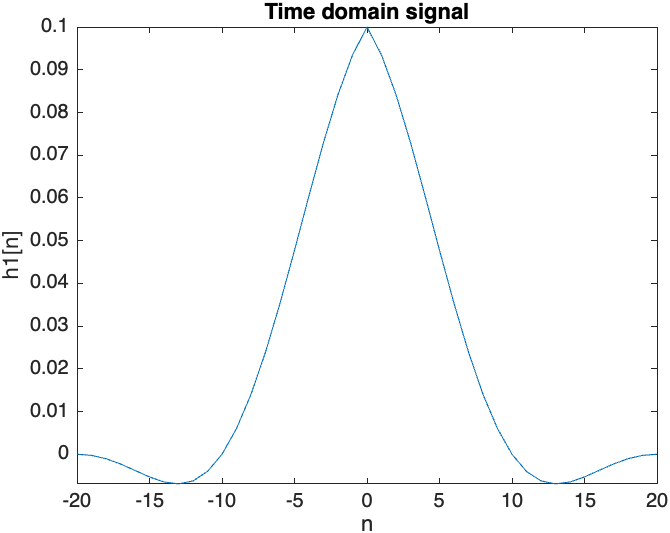
\includegraphics[width=0.75\linewidth]{13.png}
\end{figure}
\begin{figure} [H]
    \centering
    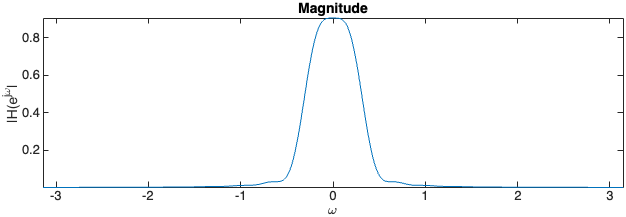
\includegraphics[width=0.75\linewidth]{14.png}
\end{figure}
\begin{figure} [H]
    \centering
    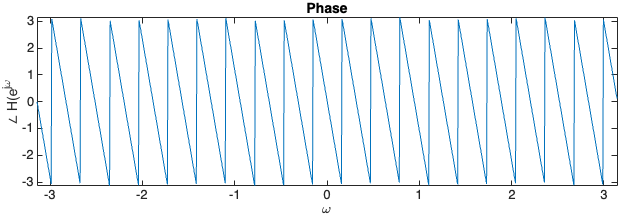
\includegraphics[width=0.75\linewidth]{15.png}
\end{figure}

Finally, for $n_0=50$, we can observe:
\begin{figure} [H]
    \centering
    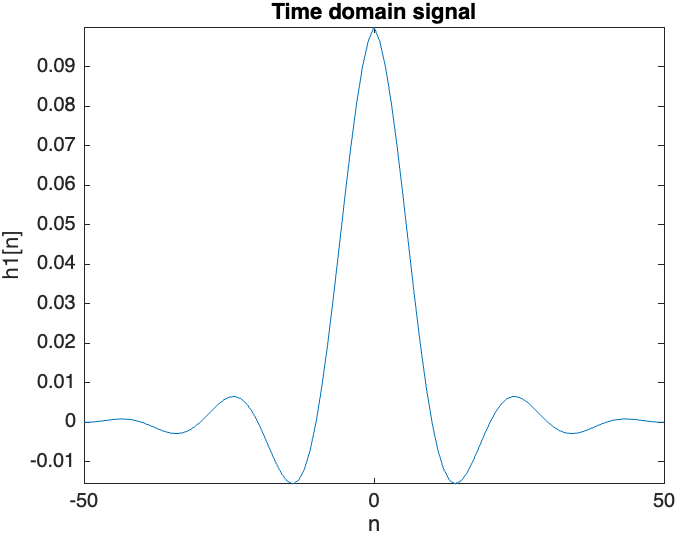
\includegraphics[width=0.75\linewidth]{16.png}
\end{figure}
\begin{figure} [H]
    \centering
    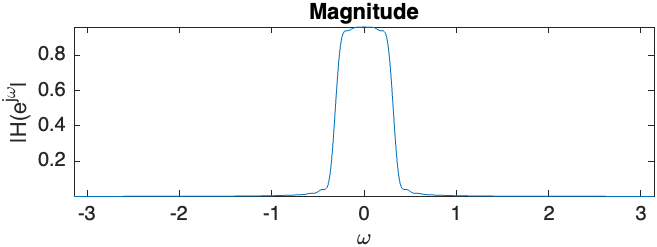
\includegraphics[width=0.75\linewidth]{17.png}
\end{figure}
\begin{figure} [H]
    \centering
    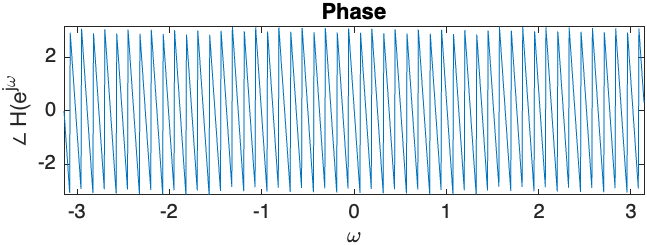
\includegraphics[width=0.75\linewidth]{18.png}
\end{figure}
We can see that the triangular pulse seems to be a much better option to approximate $|H_0(e^{j\omega})|$, primarily as we avoid the Gibbs phenomenon, which was much more apparent in \textbf{a)}. This is evident in the phase plot, which is comparatively much more consistent than it was for the rectangular plot, which had a slightly less steep slope near $\omega=0$.
\begin{minted}[frame=single, fontsize=\small, linenos, bgcolor=white]{matlab}
clear;
% h1[n]=h0[n-n0]r[n-n0]

n0 = 10;
n = -n0:n0;
h0 = sinc(n/10)/10;

t = (1-abs(n)/n0).*(abs(n)<=n0);
h1 = h0.*t;

subplot(1, 1, 1);
plot(n, h1);
xlabel('n');
ylabel('h1[n]');
axis tight;
title('Time domain signal')

windowed_resp = h1;

N_fft = 1024;

% fftshift shifts the zero - frequency to center of the array
impulse_resp_fft = fftshift(fft(windowed_resp, N_fft));

% Discrete frequencies
freqs = linspace(-pi, pi, N_fft);
fig1 = figure;

subplot(2, 1, 1);
plot(freqs, abs(impulse_resp_fft));
xlabel('\omega');
ylabel('|H(e^{j\omega}|');
axis tight;
title('Magnitude');

subplot(2, 1, 2);
plot(freqs, angle(impulse_resp_fft));
xlabel('\omega');
ylabel('\angle H(e^{j\omega}');
axis tight;
title('Phase');
\end{minted}

\item Here, we create a chirp signal of length $N=1000$ such that the frequency is $\omega_{\text{init}}=\frac{\pi}{30}$ at $n=0$, and the final frequency $\omega_{\text{final}}=\frac{\pi}{5}$ at $n=999$. Our plot for the chirp signal is shown below:
\begin{figure} [H]
    \centering
    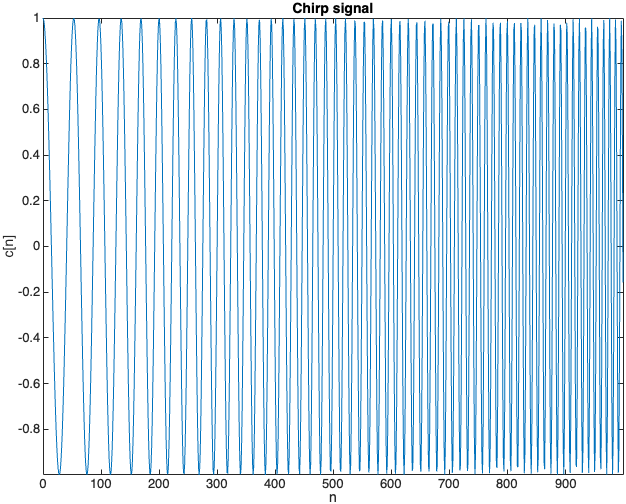
\includegraphics[width=0.75\linewidth]{19.png}
\end{figure}
Performing the convolution with $n_0=10$, we see:
\begin{figure} [H]
    \centering
    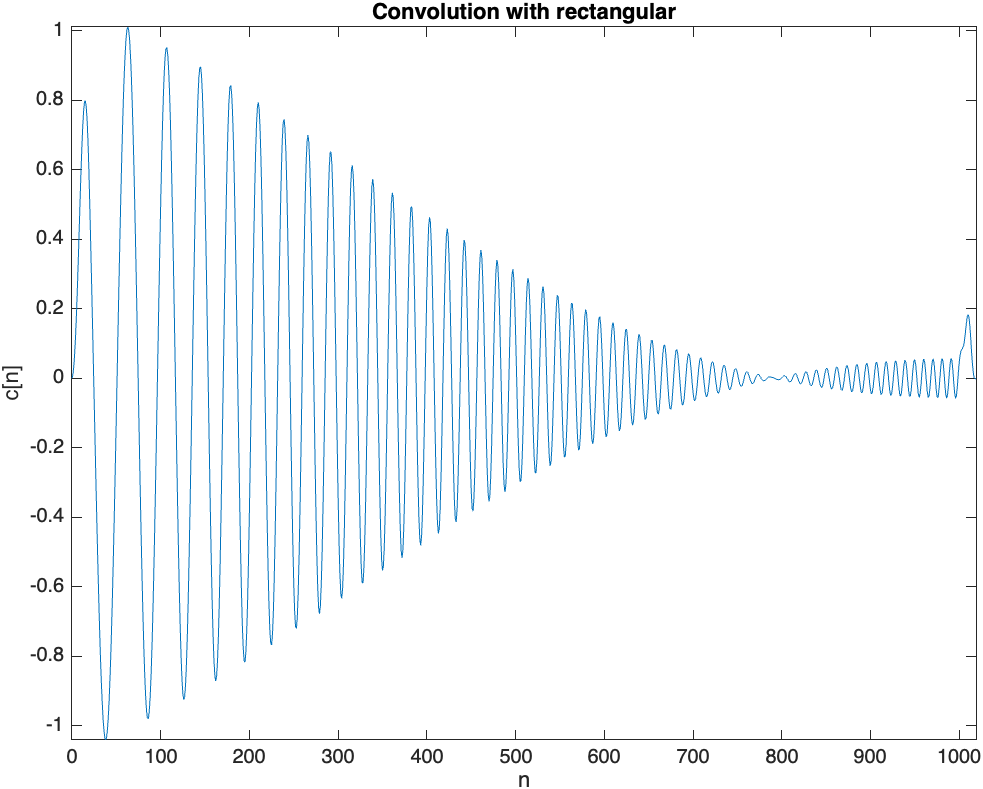
\includegraphics[width=0.75\linewidth]{20.png}
\end{figure}
\begin{figure} [H]
    \centering
    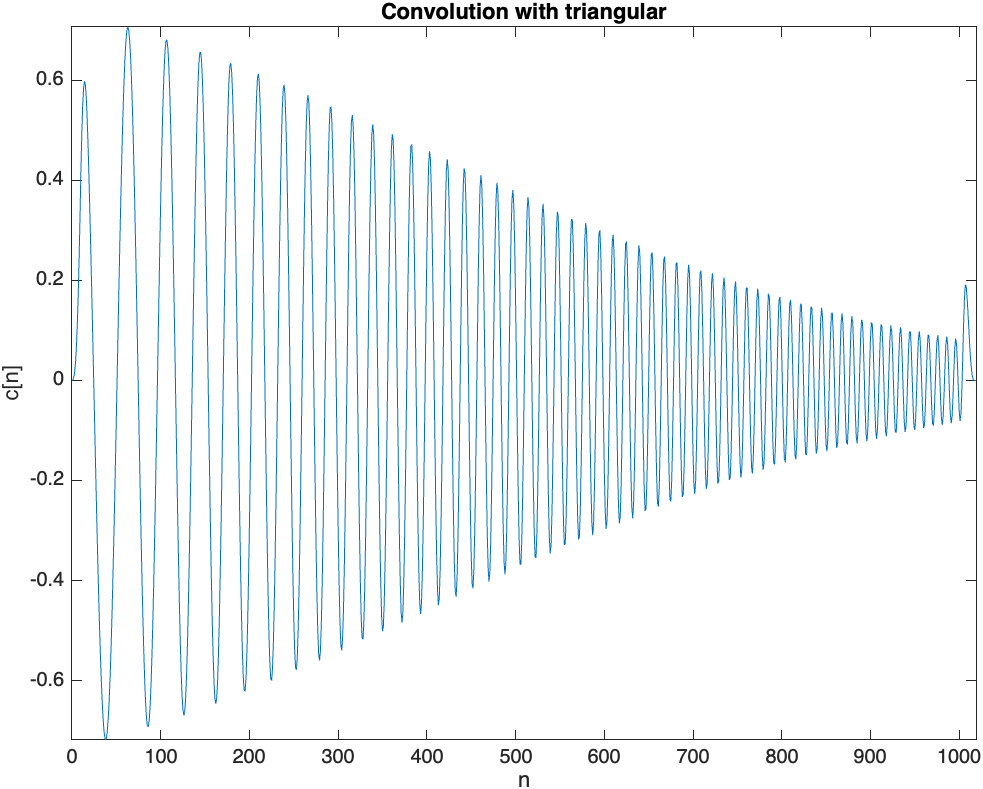
\includegraphics[width=0.75\linewidth]{21.png}
\end{figure}
For $n_0=20$, we see:
\begin{figure} [H]
    \centering
    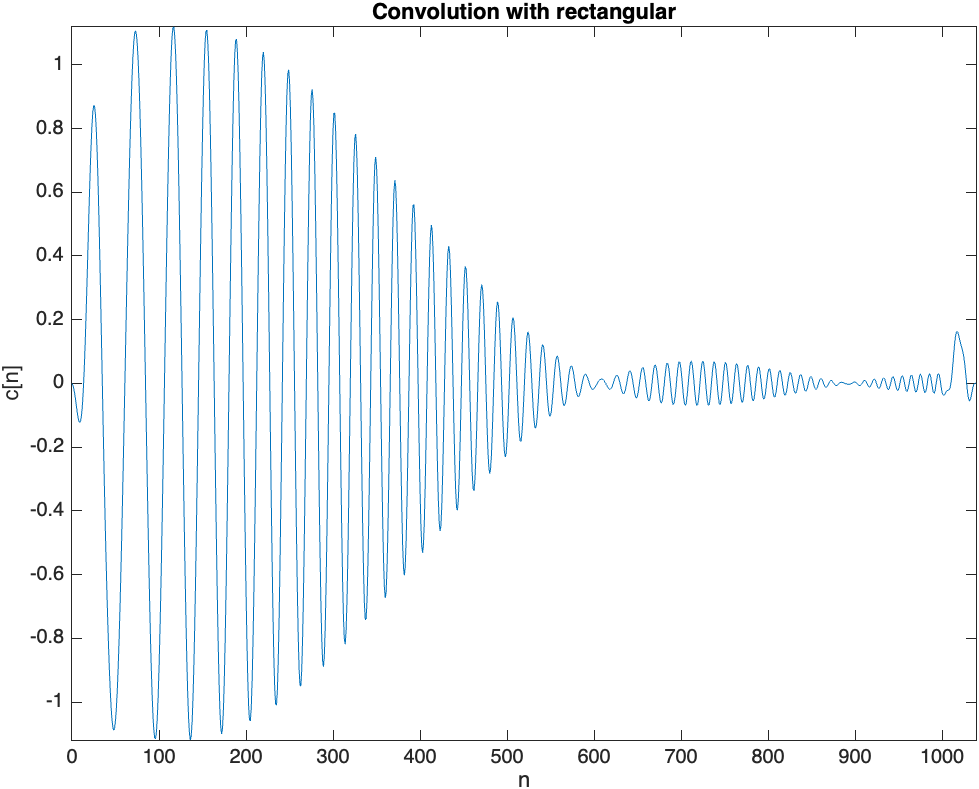
\includegraphics[width=0.75\linewidth]{22.png}
\end{figure}
\begin{figure} [H]
    \centering
    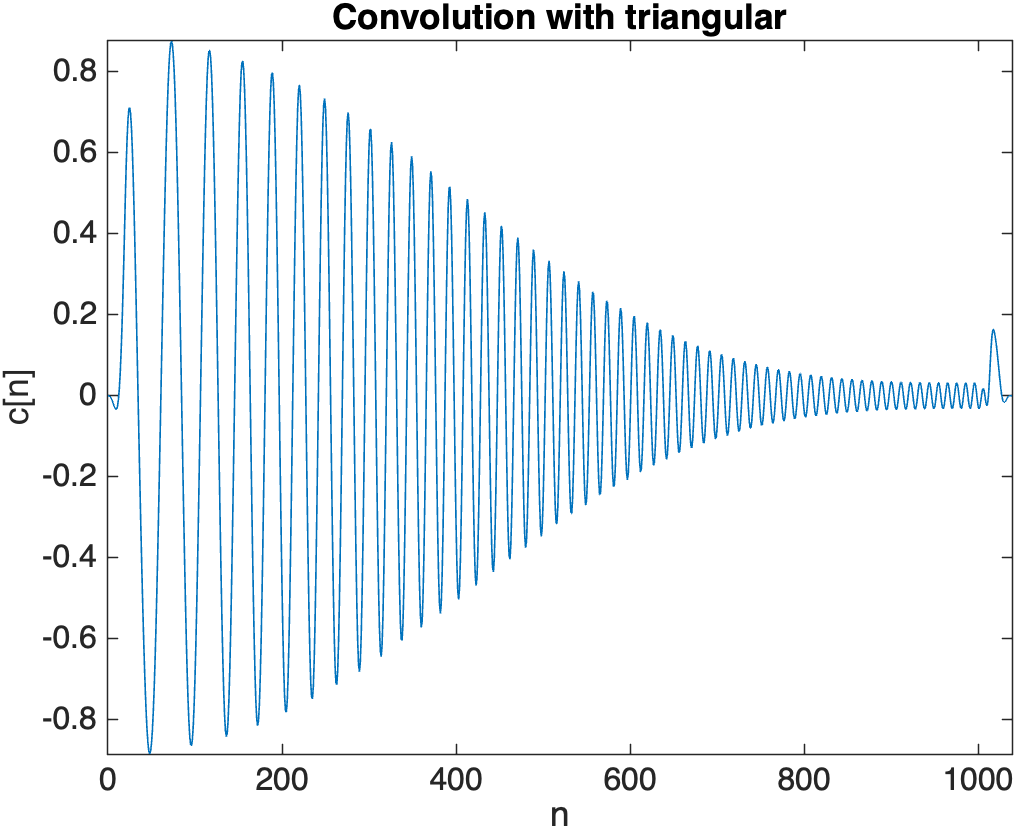
\includegraphics[width=0.75\linewidth]{23.png}
\end{figure}
And for $n_0=50$, we see:
\begin{figure} [H]
    \centering
    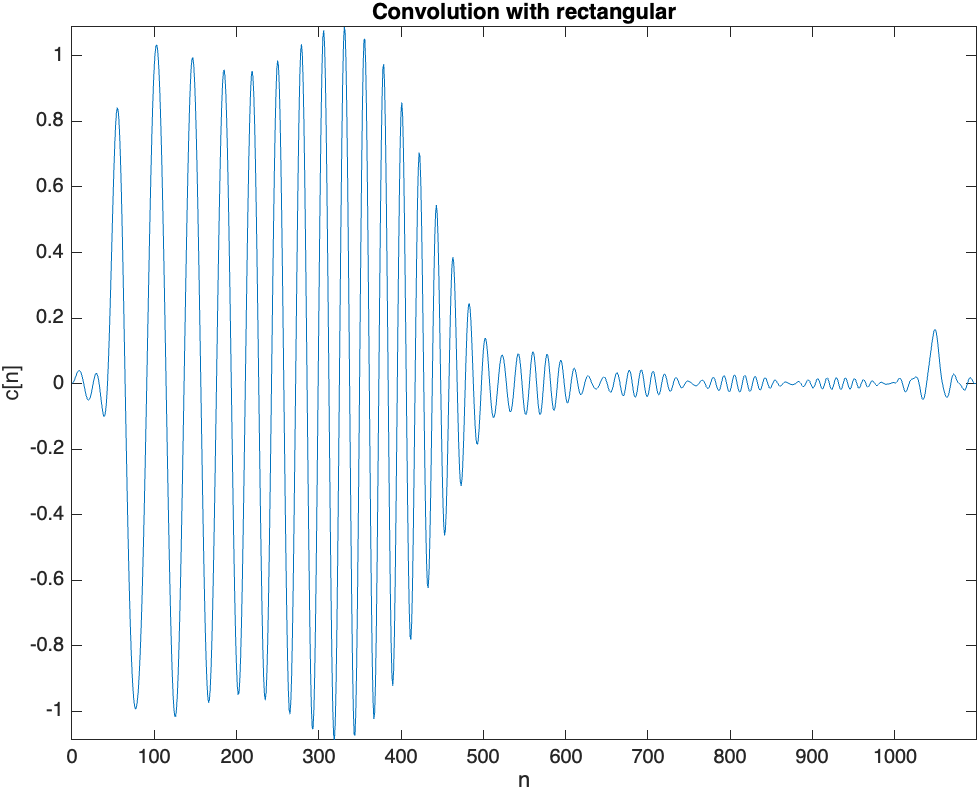
\includegraphics[width=0.75\linewidth]{25.png}
\end{figure}
\begin{figure} [H]
    \centering
    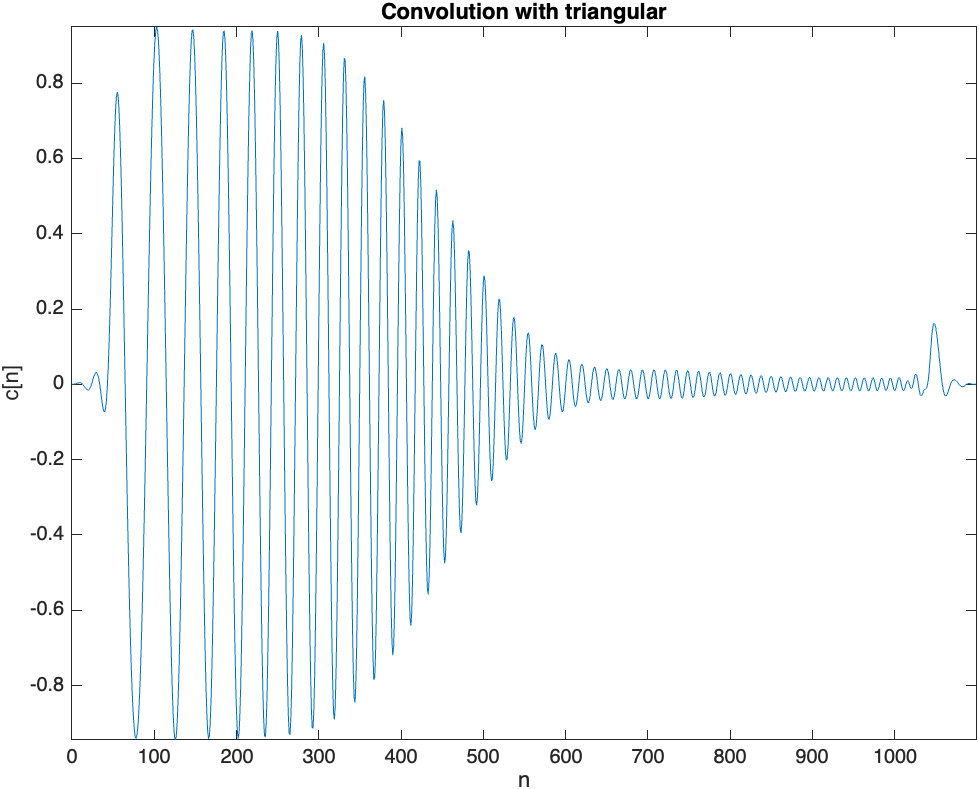
\includegraphics[width=0.75\linewidth]{24.png}
\end{figure}
We can then determine that performing the convolution between the chirp signal and our impulse responses effectively acts as a filter for the chirp signal, decreasing the amplitude of the signal as the frequency increases. This is easily seen through comparing with our earlier observations of the Gibbs phenomenon being more present with the rectangular pulse, which is also visible by the unstable amplitude as the frequency increases in its convolution with the chirp signal. On the other hand, the triangular pulse, which did not exhibit the Gibbs phenomenon to the same degree as the rectangular pulse, dampens the amplitude at higher frequencies more smoothly across the frequency range, yet not being as effective.
\begin{minted}[frame=single, fontsize=\small, linenos, bgcolor=white]{matlab}
clear;
% h1[n]=h0[n-n0]r[n-n0]

n0 = 50;
n = -n0:n0;
h0 = sinc(n/10)/10;

r1 = ones(size(n));
h1 = h0.*r1;

subplot(1, 1, 1);
plot(n, h1);
xlabel('n');
ylabel('h1[n]');
axis tight;
title('Time domain signal')

windowed_resp = h1;

N_fft = 1024;

impulse_resp_fft = fftshift(fft(windowed_resp, N_fft));

% Discrete frequencies
freqs = linspace(-pi, pi, N_fft);
fig1 = figure;

subplot(2, 1, 1);
plot(freqs, abs(impulse_resp_fft));
xlabel('\omega');
ylabel('|H(e^{j\omega}|');
axis tight;
title('Magnitude');

subplot(2, 1, 2);
plot(freqs, angle(impulse_resp_fft));
xlabel('\omega');
ylabel('\angle H(e^{j\omega}');
axis tight;
title('Phase');

t1 = (1-abs(n)/n0).*(abs(n)<=n0);
h1 = h0.*t1;

subplot(1, 1, 1);
plot(n, h1);
xlabel('n');
ylabel('h1[n]');
axis tight;
title('Time domain signal')

windowed_resp = h1;

N_fft = 1024;

impulse_resp_fft = fftshift(fft(windowed_resp, N_fft));

% Discrete frequencies
freqs = linspace(-pi, pi, N_fft);
fig1 = figure;

subplot(2, 1, 1);
plot(freqs, abs(impulse_resp_fft));
xlabel('\omega');
ylabel('|H(e^{j\omega}|');
axis tight;
title('Magnitude');

subplot(2, 1, 2);
plot(freqs, angle(impulse_resp_fft));
xlabel('\omega');
ylabel('\angle H(e^{j\omega}');
axis tight;
title('Phase');

N = 1000;
n = 0:N-1;

% converting to Hz
f0 = (pi/30)/(2*pi);
f1 = (pi/5)/(2*pi);

c1 = chirp(n, f0, n(end), f1, 'linear');

figure;
plot(n, c1);
xlabel('n');
ylabel('c[n]');
title('Chirp signal');
axis tight;

figure;
plot(0:N+n0*2-1, conv(c1, h0.*r1));
xlabel('n');
ylabel('c[n]');
title('Convolution with rectangular');
axis tight;

figure;
plot(0:N+n0*2-1, conv(c1, h0.*t1));
xlabel('n');
ylabel('c[n]');
title('Convolution with triangular');
axis tight;
\end{minted}

\end{enumerate}
\end{document}